\resizebox{7cm}{4.4cm}{
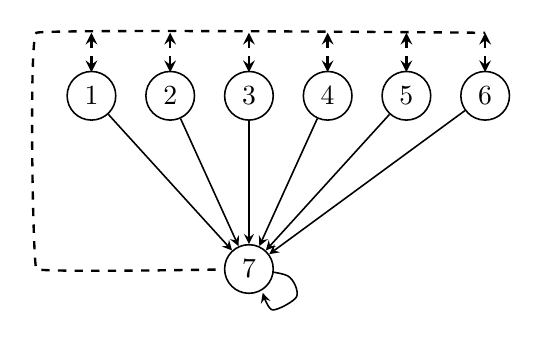
\begin{tikzpicture}[smooth]
\node[coordinate] (origin) at (0.3,0) {};
\node[coordinate] (num7) at (3,0) {};
\node[coordinate] (num1) at (1,2.5) {};
\path (num7) ++ (-10:0.5cm) node (num7_bright1) [coordinate] {};
\path (num7) ++ (-30:0.7cm) node (num7_bright2) [coordinate] {};
\path (num7) ++ (-60:0.35cm) node (num7_bright3) [coordinate] {};
\path (num7) ++ (-60:0.6cm) node (num7_bright4) [coordinate] {};
\path (origin) ++ (90:3cm) node (origin_above) [coordinate] {};
\path (origin_above) ++ (0:5.7cm) node (origin_aright) [coordinate] {};
\path (num1) ++ (90:0.5cm) node (num1_a) [coordinate] {};
\path (num1) ++ (-90:0.3cm) node (num1_b) [coordinate] {};

\path (num1) ++ (0:1cm) node (num2) [coordinate] {};
\path (num1_a) ++ (0:1cm) node (num2_a) [coordinate] {};
\path (num1_b) ++ (0:1cm) node (num2_b) [coordinate] {};
\path (num2) ++ (0:1cm) node (num3) [coordinate] {};
\path (num2_a) ++ (0:1cm) node (num3_a) [coordinate] {};
\path (num2_b) ++ (0:1cm) node (num3_b) [coordinate] {};
\path (num3) ++ (0:1cm) node (num4) [coordinate] {};
\path (num3_a) ++ (0:1cm) node (num4_a) [coordinate] {};
\path (num3_b) ++ (0:1cm) node (num4_b) [coordinate] {};
\path (num4) ++ (0:1cm) node (num5) [coordinate] {};
\path (num4_a) ++ (0:1cm) node (num5_a) [coordinate] {};
\path (num4_b) ++ (0:1cm) node (num5_b) [coordinate] {};
\path (num5) ++ (0:1cm) node (num6) [coordinate] {};
\path (num5_a) ++ (0:1cm) node (num6_a) [coordinate] {};
\path (num5_b) ++ (0:1cm) node (num6_b) [coordinate] {};


%\draw[->](0,0) -- (1,1);
%\draw[dashed,line width = 0.03cm] (0,0) -- (1,1);
 %\fill (0.5,0.5) circle (0.5);
 %\draw[shape=circle,fill=white,draw=black] (a) at (num7) {7};

 
\draw[dashed,line width = 0.03cm,xshift=3cm] plot[tension=0.06]
coordinates{(num7) (origin) (origin_above) (origin_aright)}; 

\draw[->,>=stealth,line width = 0.02cm,xshift=3cm] plot[tension=0.5]
coordinates{(num7) (num7_bright1) (num7_bright2)(num7_bright4) (num7_bright3)};
 
\node[line width = 0.02cm,shape=circle,fill=white,draw=black] (g) at (num7) {7};



\draw[<->,>=stealth,dashed,line width = 0.03cm,] (num1) -- (num1_a) ;
\node[line width = 0.02cm,shape=circle,fill=white,draw=black] (a) at (num1_b) {1};
\draw[<->,>=stealth,dashed,line width = 0.03cm,] (num2) -- (num2_a) ;
\node[line width = 0.02cm,shape=circle,fill=white,draw=black] (b) at (num2_b) {2};
\draw[<->,>=stealth,dashed,line width = 0.03cm,] (num3) -- (num3_a) ;
\node[line width = 0.02cm,shape=circle,fill=white,draw=black] (c) at (num3_b) {3};
\draw[<->,>=stealth,dashed,line width = 0.03cm,] (num4) -- (num4_a) ;
\node[line width = 0.02cm,shape=circle,fill=white,draw=black] (d) at (num4_b) {4};
\draw[<->,>=stealth,dashed,line width = 0.03cm,] (num5) -- (num5_a) ;
\node[line width = 0.02cm,shape=circle,fill=white,draw=black] (e) at (num5_b) {5};
\draw[<->,>=stealth,dashed,line width = 0.03cm,] (num6) -- (num6_a) ;
\node[line width = 0.02cm,shape=circle,fill=white,draw=black] (f) at (num6_b) {6};

\draw[->,>=stealth,line width = 0.02cm] (a)--(g);
\draw[->,>=stealth,line width = 0.02cm] (b)--(g);
\draw[->,>=stealth,line width = 0.02cm] (c)--(g);
\draw[->,>=stealth,line width = 0.02cm] (d)--(g);
\draw[->,>=stealth,line width = 0.02cm] (e)--(g);
\draw[->,>=stealth,line width = 0.02cm] (f)--(g);
\end{tikzpicture}
}

